\documentclass[11pt,a4paper]{article}

% ---------- Paquetes ----------
\usepackage[utf8]{inputenc}
\usepackage[T1]{fontenc}
\usepackage[spanish,es-tabla]{babel}
\usepackage[margin=2cm]{geometry}
\usepackage{graphicx}
\usepackage{booktabs}
\usepackage{longtable}
\usepackage{array}
\usepackage{xcolor}
\usepackage{setspace}
\usepackage{float}
\usepackage{fancyhdr}
\usepackage[hidelinks]{hyperref}

\setstretch{1.1}
\setlength{\parindent}{0pt}
\setlength{\parskip}{6pt}

\pagestyle{fancy}
\fancyhf{}
\setlength{\headheight}{14pt}
\lhead{\small TA-IND-01: Banca móvil del Banco Pichincha}
\rhead{\small Ingeniería de Requerimientos (ISR-401)}
\cfoot{\small Página \thepage}

\title{Requisitos bien formados según ISO/IEC/IEEE 29148:2018\\
\large Análisis de la banca móvil del Banco Pichincha}
\author{Erick Ariel Monserrate Ochoa\\
Carrera de Software, 4.\textsuperscript{o} nivel, paralelo A\\
Ingeniería de Requerimientos (ISR-401)\\
Universidad Técnica Estatal de Quevedo}
\date{11 de noviembre de 2026}

\begin{document}
\maketitle

% =====================================================
\section{Sistema elegido}
\label{sec:sistema}
La banca móvil del Banco Pichincha es una aplicación para teléfonos celulares que permite a los clientes del banco gestionar y controlar sus cuentas (agregar contactos de destinatarios nuevos o frecuentes, consultar el saldo disponible en tiempo real, revisar el historial de movimientos filtrando por fechas y compartir comprobantes de operación), realizar transferencias hacia cuentas del mismo banco o de otras entidades y pagar servicios. Sus usuarios son las personas asociadas a la entidad, quienes la utilizan a diario desde el celular. El uso frecuente de las transferencias se ha vuelto un hábito, ya que evita retirar efectivo con regularidad. Este informe se centra en la función de transferencias de dinero.

% =====================================================
\section{Resumen analítico de la norma}
\label{sec:resumen}
La norma ISO/IEC/IEEE 29148:2018 establece las reglas y procesos para transformar las necesidades de los usuarios y partes interesadas en requisitos técnicos claros, consistentes y verificables durante el ciclo de vida del software~\cite{iso29148}. Su aplicación evita que los programadores y evaluadores interpreten de forma distinta lo que el sistema debe hacer, fundamentando la ingeniería de requisitos sobre bases objetivas~\cite{pohl2025}.

\subsection{Requisito bien formado}
Según la cláusula 5.2.4~\cite{iso29148}, un requisito bien formado se construye identificando una condición o evento disparador («Cuando...»), el sujeto que realiza la acción («el sistema»), el verbo auxiliar modal de obligatoriedad («debe») y la acción observable junto con sus restricciones o umbrales medibles.

De acuerdo con las convenciones de lenguaje de la norma (cláusulas 1 y 5.2.4)~\cite{iso29148}, el verbo «debe» (\textit{shall}) expresa un requisito obligatorio y vinculante, que siempre tiene que verificarse. El verbo «debería» (\textit{should}) indica una recomendación: algo deseable, pero no necesariamente obligatorio. El verbo «puede» (\textit{may}) expresa algo opcional, es decir, que el sistema está autorizado o permitido a realizar.

\subsection{Características de un requisito individual}
La cláusula 5.2.5~\cite{iso29148} define las nueve características que debe cumplir cada requisito por separado:
\begin{itemize}
  \item \textbf{Necesario:} responde a una necesidad real del usuario o a una regla del negocio que, si se elimina, deja incompleto el propósito del sistema. Por ejemplo: «El sistema debe permitir al usuario pagar sus servicios».
  \item \textbf{Apropiado:} se mantiene en el nivel de qué debe hacer el sistema para el usuario sin meterse a detallar cómo programarlo por dentro (tablas, clases o variables). Por ejemplo: «El sistema debe permitir al usuario ver el historial de movimientos de su cuenta».
  \item \textbf{No ambiguo:} tiene una sola forma de interpretarse. Por ejemplo: «Cuando el usuario ingresa un monto a transferir a otro banco, el sistema debe mostrar el costo de \$0{,}41 antes de continuar», en lugar de decir «mostrará una comisión baja».
  \item \textbf{Completo:} a nivel individual, el enunciado incluye toda la información, datos de entrada y condiciones necesarias para entender qué se espera sin depender de suposiciones externas. Por ejemplo: «Cuando el usuario paga un servicio, el sistema debe debitar de su cuenta el valor pagado».
  \item \textbf{Singular:} expresa un solo objetivo o acción a la vez, sin mezclar varias tareas con la conjunción «y». Por ejemplo: «Cuando la transferencia se completa correctamente, el sistema debe mostrar el mensaje "¡Transferencia exitosa!"», separándolo del requisito de ocultar los dígitos de la cuenta.
  \item \textbf{Factible:} puede construirse en la práctica con la tecnología actual, el tiempo y el presupuesto del proyecto. Por ejemplo: «El sistema debe mostrar el resultado de la transferencia en menos de 10 segundos», ya que exigir 0 milisegundos bajo redes móviles sería técnicamente imposible.
  \item \textbf{Verificable:} cuenta con una prueba real que permite comprobar si se cumplió o no. Por ejemplo, el primer borrador de RQ-08 decía que «la app demorará 10 segundos en realizarla», lo cual no fijaba un límite máximo medible; al corregirlo a «mostrar el resultado en menos de 10 segundos», se puede verificar con un cronómetro.
  \item \textbf{Correcto:} refleja con exactitud lo que el usuario o las reglas del banco exigen, sin datos equivocados. Por ejemplo, en el primer borrador de RQ-02 se escribió «realizar un depósito» cuando el flujo real de la aplicación corresponde a una «transferencia».
  \item \textbf{Conforme:} sigue la plantilla gramatical y el estilo formal definidos (condición + «el sistema debe» + acción), evitando hablarle al usuario en segunda persona. Por ejemplo, sustituir «cuando ingreses en la app te pedirá huella» por «Cuando el usuario inicia sesión, el sistema debe solicitar autenticación biométrica».
\end{itemize}

\subsection{Características de un conjunto de requisitos}
Según la cláusula 5.2.6~\cite{iso29148}, el conjunto de requisitos debe ser \textbf{consistente}: ningún requisito contradice a otro, ni en las funciones ni en las reglas de negocio, y se usan los mismos términos para referirse a los mismos objetos. Debe ser \textbf{completo}: el conjunto cubre todos los escenarios, funciones e impactos sin que falten piezas esenciales ni queden elementos «por definir» para que el sistema funcione. Debe ser \textbf{viable} (\textit{affordable}): todo el conjunto puede construirse dentro del presupuesto, el equipo y el tiempo realmente disponibles. Debe estar \textbf{acotado} (\textit{bounded}): mantiene el alcance dentro de las fronteras del sistema sin agregar funciones innecesarias. Además, el conjunto debe ser \textbf{comprensible} para quienes lo leen y \textbf{validable} para comprobar que cumple las metas de los usuarios en su entorno real.

\subsection{Términos ambiguos}
La cláusula 5.2.7~\cite{iso29148} indica que se deben evitar las palabras subjetivas, como «bien», «mal», «rápido», «intuitivo», «seguro» y «eficiente», así como los comodines, como «etcétera» o «según sea necesario», y los absolutos sin contexto de prueba. La razón es que lo que una persona considera «bien» otra puede considerarlo «mal», y esas palabras impiden diseñar una prueba técnica objetiva. Todo término subjetivo debe sustituirse por números, pasos o reglas claras. Por ejemplo, en mis primeros borradores de RQ-06 y RQ-07 escribí «cuando se realizó una transferencia bien» y «cuando se realizó una transferencia mal»; ambos términos tuvieron que cambiarse por condiciones concretas (completarse correctamente o no poderse completar) y por los textos exactos que muestra la pantalla («¡Transferencia exitosa!» y «Algo salió mal»).

% =====================================================
\section{Glosario}
\label{sec:glosario}
{\footnotesize
\setlength{\tabcolsep}{3pt}
\renewcommand{\arraystretch}{1.25}
\begin{longtable}{>{\raggedright\arraybackslash}p{3cm}
                  >{\raggedright\arraybackslash}p{6.4cm}
                  >{\raggedright\arraybackslash}p{6.4cm}}
\caption{Glosario de términos de la cláusula 3 de ISO/IEC/IEEE 29148.}\label{tab:glosario}\\
\toprule
\textbf{Término} & \textbf{Definición parafraseada} & \textbf{Ejemplo en la banca móvil}\\
\midrule
\endfirsthead
\toprule
\textbf{Término} & \textbf{Definición parafraseada} & \textbf{Ejemplo en la banca móvil}\\
\midrule
\endhead
1. Requisito (\textit{Requirement}, 3.1.18) & Enunciado que traduce una necesidad o condición operativa que el sistema debe cumplir de forma verificable. & Cuando el usuario transfiere a otro banco, el sistema debe mostrar el costo de \$0{,}41 antes de continuar.\\
2. Parte interesada (\textit{Stakeholder}, 3.1.26) & Persona, grupo u organización que tiene un interés o se ve afectada por el funcionamiento del sistema. & El cliente titular de la cuenta (usuario «ERICK5312»), el destinatario de la transferencia y el Banco Pichincha.\\
3. Verificación (\textit{Verification}, 3.1.30) & Prueba objetiva que demuestra que el sistema cumple exactamente con los requisitos especificados. & Intentar tomar captura de pantalla en 5 vistas distintas de la app para comprobar que el sistema las bloquea todas.\\
4. Validación (\textit{Validation}, 3.1.29) & Confirmación de que el sistema construido realmente sirve para lo que el usuario necesita en su entorno diario. & Confirmar que un cliente puede transferir \$10{,}00 a la cuenta de su mamá desde el celular sin ir al cajero.\\
5. Restricción (\textit{Constraint}, 3.1.8) & Límite externo impuesto al sistema que restringe cómo se puede diseñar o utilizar. & La prohibición de realizar capturas de pantalla dentro de la aplicación por políticas de seguridad bancaria.\\
6. Requisito funcional (\textit{Functional requirement}, 3.1.13) & Requisito que define una acción, cálculo o respuesta concreta que el sistema debe ejecutar. & Verificar que un número de cuenta del Banco Pichincha exista antes de permitir continuar con el envío.\\
7. Requisito de desempeño (\textit{Performance requirement}, 3.1.17) & Requisito que fija un límite cuantitativo de tiempo, velocidad o capacidad sobre una función del sistema. & Mostrar en pantalla el resultado de la transferencia en menos de 10 segundos tras haberla aceptado.\\
8. Trazabilidad (\textit{Traceability}, 3.1.28) & Capacidad de conectar cada requisito con su origen, con las pantallas del sistema y con sus pruebas de aceptación. & Relacionar el requisito RQ-11 con la captura del comprobante (Figura~\ref{fig:comprobante}) y su criterio de prueba.\\
9. Requisito de interfaz (\textit{Interface requirement}, 3.1.14) & Especificación de cómo el sistema se comunica o intercambia información con otros sistemas externos. & Consultar y mostrar el listado de bancos externos que mantienen convenio de transferencia directa.\\
10. Requisito de calidad / no funcional (\textit{Non-functional requirement}, 3.1.16) & Propiedad de calidad que indica qué tan seguro, usable o confiable debe ser el sistema al operar. & Ocultar los dígitos de los números de cuenta en el comprobante dejando visibles únicamente los cuatro últimos.\\
\bottomrule
\end{longtable}
}

% =====================================================
\section{Evidencias del sistema}
\label{sec:evidencias}
Dado que la aplicación bloquea las capturas de pantalla en todas sus vistas, las evidencias se obtuvieron fotografiando la pantalla con otro dispositivo, a excepción de la Figura~\ref{fig:comprobante}, cuya imagen fue exportada directamente mediante la opción «Compartir comprobante» de la propia aplicación. Las Figuras~\ref{fig:auth}, \ref{fig:tarifa}, \ref{fig:comprobante}, \ref{fig:historial} y \ref{fig:bancos} respaldan los requisitos de la Sección~\ref{sec:requisitos}. El identificador «ERICK5312» corresponde al usuario del autor. Los datos de terceros y los números de cuenta fueron cubiertos.

\begin{figure}[H]
  \centering
  \begin{minipage}[t]{0.48\textwidth}
    \centering
    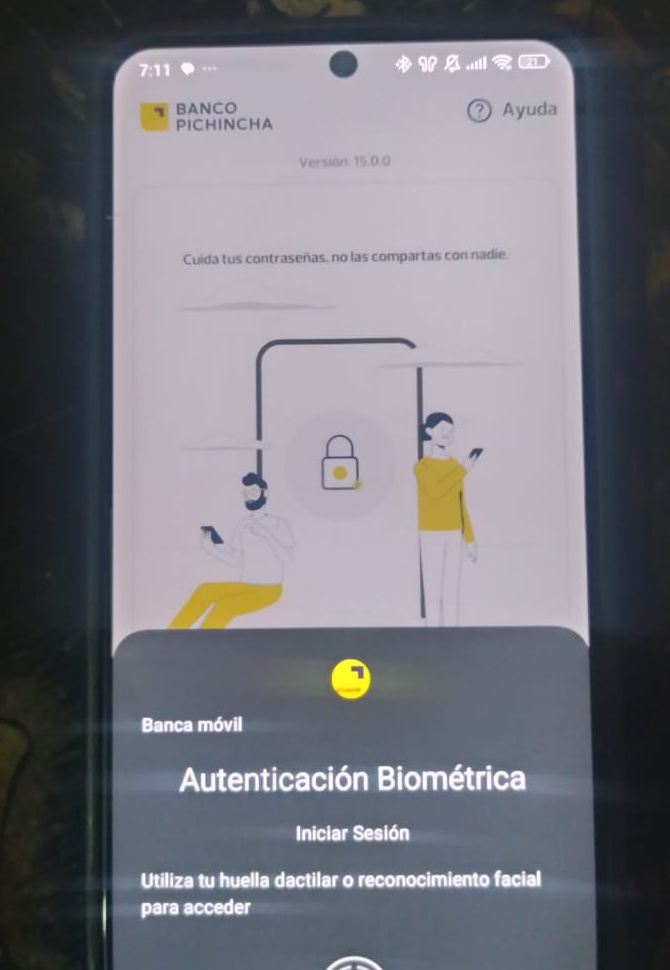
\includegraphics[angle=-90,height=6.5cm]{figuras/autenticacion.jpeg}
    \caption{Inicio de sesión con autenticación biométrica.}
    \label{fig:auth}
  \end{minipage}\hfill
  \begin{minipage}[t]{0.48\textwidth}
    \centering
    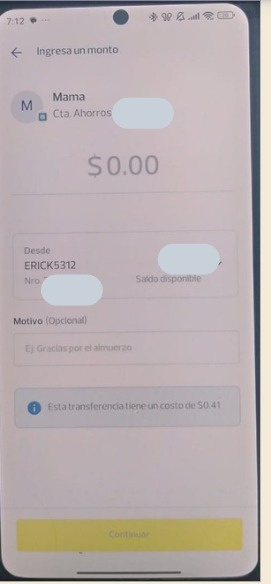
\includegraphics[height=6.5cm]{figuras/monto_tarifa.jpeg}
    \caption{Pantalla del monto con el costo de \$0{,}41.}
    \label{fig:tarifa}
  \end{minipage}
\end{figure}

\begin{figure}[H]
  \centering
  \begin{minipage}[t]{0.48\textwidth}
    \centering
    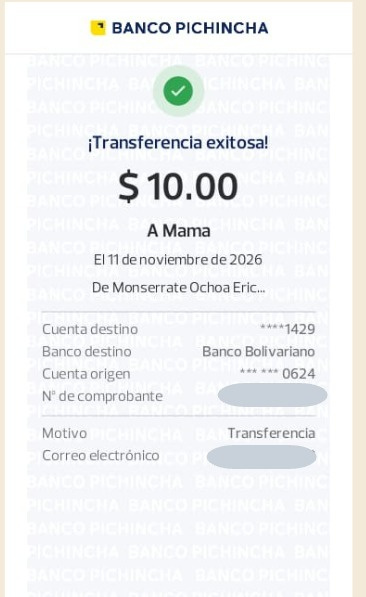
\includegraphics[height=6.5cm]{figuras/comprobante_exitoso.jpeg}
    \caption{Comprobante de transferencia exitosa.}
    \label{fig:comprobante}
  \end{minipage}\hfill
  \begin{minipage}[t]{0.48\textwidth}
    \centering
    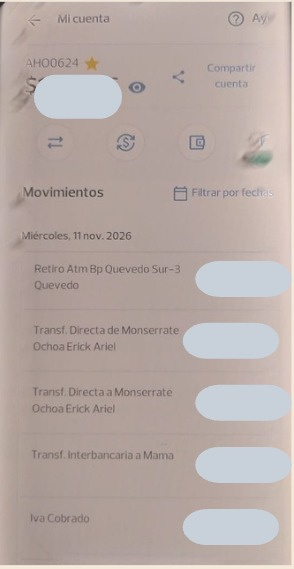
\includegraphics[height=6.5cm]{figuras/movimientos_historial.jpeg}
    \caption{Historial de movimientos de la cuenta.}
    \label{fig:historial}
  \end{minipage}
\end{figure}

\begin{figure}[H]
  \centering
  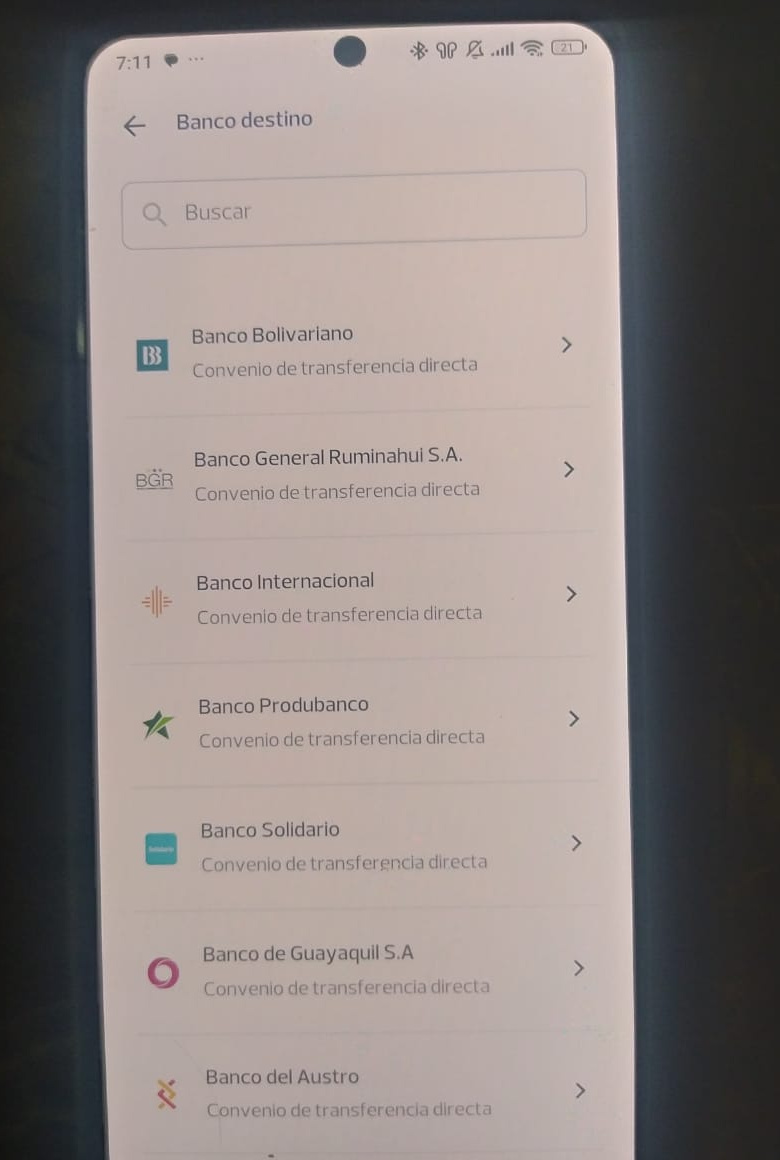
\includegraphics[angle=-90,height=6.5cm]{figuras/bancos_spi.jpeg}
  \caption{Lista de bancos destino con buscador.}
  \label{fig:bancos}
\end{figure}

% =====================================================
\section{Requisitos del sistema}
\label{sec:requisitos}
La Tabla~\ref{tab:requisitos} presenta quince requisitos de la función de transferencias de la banca móvil, distribuidos en cinco tipos de la cláusula 5.2 de ISO/IEC/IEEE 29148:2018: funcional, desempeño, interfaz externa, calidad y usabilidad (calidad en uso)~\cite{iso29148}. Los requisitos de calidad y desempeño se clasifican según las características y subcaracterísticas de ISO/IEC 25010:2023~\cite{iso25010}.

{\footnotesize
\setlength{\tabcolsep}{3pt}
\renewcommand{\arraystretch}{1.25}
\begin{longtable}{>{\raggedright\arraybackslash}p{1.2cm}
                  >{\raggedright\arraybackslash}p{4.6cm}
                  >{\raggedright\arraybackslash}p{1.7cm}
                  >{\raggedright\arraybackslash}p{2.1cm}
                  >{\raggedright\arraybackslash}p{2.3cm}
                  >{\raggedright\arraybackslash}p{3.2cm}}
\caption{Clasificación de los requisitos de la banca móvil.}\label{tab:requisitos}\\
\toprule
\textbf{ID} & \textbf{Enunciado} & \textbf{Tipo} & \textbf{Caract. ISO/IEC 25010} & \textbf{Métrica} & \textbf{Criterio de aceptación}\\
\midrule
\endfirsthead
\toprule
\textbf{ID} & \textbf{Enunciado} & \textbf{Tipo} & \textbf{Caract. ISO/IEC 25010} & \textbf{Métrica} & \textbf{Criterio de aceptación}\\
\midrule
\endhead
RQ-01 & Cuando el usuario ingresa el monto de una transferencia a otro banco, el sistema debe mostrar el costo de \$0{,}41 antes de que el usuario pulse «Continuar». & Funcional & N/A & --- & El costo de \$0{,}41 aparece en la pantalla del monto, antes del botón «Continuar».\\
RQ-02 & Cuando el usuario realiza una transferencia a una cuenta del mismo banco, el sistema debe solicitar el tipo de cuenta destino (ahorros o corriente). & Funcional & N/A & --- & Al transferir a una cuenta del mismo banco, la aplicación solicita el tipo de cuenta.\\
RQ-03 & Cuando el usuario ingresa un número de cuenta destino del Banco Pichincha, el sistema debe verificar que la cuenta exista. & Funcional & N/A & --- & Con un número de cuenta del banco, la aplicación verifica su existencia antes de continuar.\\
RQ-04 & Cuando el número de cuenta ingresado no existe, el sistema debe mostrar el mensaje «Cuenta inválida. Revisa el número de cuenta e inténtalo nuevamente». & Funcional & N/A & --- & Con un número inexistente, la aplicación muestra el mensaje indicado.\\
RQ-05 & Cuando el usuario confirma los datos de la transferencia, el sistema debe completar automáticamente el código de seguridad y mostrar el botón para aceptarla. & Calidad & Seguridad / Autenticidad & Cociente entre transferencias donde la clave temporal se autocompleta y transferencias confirmadas; umbral: 100\,\%. & En 3 transferencias realizadas de prueba, en las 3 el código se autocompletó y habilitó el botón de confirmación.\\
RQ-06 & Cuando la transferencia se completa correctamente, el sistema debe mostrar el mensaje «¡Transferencia exitosa!». & Funcional & N/A & --- & Al completarse la transferencia, la aplicación muestra el mensaje indicado.\\
RQ-07 & Cuando la transferencia no se puede completar, el sistema debe mostrar el mensaje «Algo salió mal». & Funcional & N/A & --- & Si la transferencia falla, la aplicación muestra el mensaje indicado.\\
RQ-08 & Cuando el usuario acepta la transferencia, el sistema debe mostrar el resultado en menos de 10 segundos. & Desempeño & Eficiencia de desempeño / Comportamiento temporal & Tiempo entre aceptar la transferencia y ver el resultado, en segundos; umbral: menor de 10 s. & En 3 pruebas de transferencia realizadas, el comprobante apareció en pantalla en menos de 4 segundos en todos los casos.\\
RQ-09 & Cuando el usuario inicia sesión, el sistema debe solicitar autenticación biométrica (huella dactilar o reconocimiento facial). & Calidad & Seguridad / Autenticidad & Cociente entre los intentos de abrir la aplicación que solicitan biometría y los intentos realizados; umbral: 100\,\%. & En 5 intentos de abrir la aplicación, en los 5 se solicitó la huella dactilar.\\
RQ-10 & Cuando el usuario intenta capturar la pantalla en cualquier vista de la aplicación, el sistema debe impedir la captura. & Calidad & Seguridad / Confidencialidad & Cociente entre intentos de captura bloqueados y el total de vistas probadas; umbral: 100\,\%. & Se intentó capturar pantalla con los botones del celular en 5 vistas distintas y en las 5 el sistema impidió la captura.\\
RQ-11 & Cuando se completa una transferencia, el sistema debe mostrar en el comprobante, como mínimo, el monto, el destinatario, la fecha, el banco destino, el motivo y el número de comprobante. & Funcional & N/A & --- & El comprobante muestra los seis datos indicados.\\
RQ-12 & Cuando el sistema muestra el comprobante, debe ocultar los dígitos de los números de cuenta, dejando visibles solo los cuatro últimos. & Calidad & Seguridad / Confidencialidad & Dígitos visibles del número de cuenta; umbral: 4. & En el comprobante generado, tanto la cuenta destino (****1429) como la de origen (*** *** 0624) muestran solo los cuatro últimos dígitos.\\
RQ-13 & Cuando el usuario selecciona «Otros bancos» al agregar una nueva cuenta, el sistema debe mostrar un buscador para encontrar el banco destino. & Usabilidad & Capacidad de interacción / Operabilidad & Presencia del campo buscador en la vista de bancos; umbral: 1 buscador visible. & Al elegir «Otros bancos», aparece el buscador en la parte superior de la lista.\\
RQ-14 & Cuando el usuario selecciona «Nueva cuenta», el sistema debe permitir elegir entre Banco Pichincha y Otros bancos. & Funcional & N/A & --- & Al elegir «Nueva cuenta», se ofrecen ambas pestañas de selección.\\
RQ-15 & Cuando el usuario selecciona «Otros bancos», el sistema debe mostrar la lista de bancos con convenio de transferencia directa. & Interfaz externa & N/A & --- & La lista de bancos aparece con la leyenda «Convenio de transferencia directa» bajo cada entidad.\\
\bottomrule
\end{longtable}
}

% =====================================================
\section{Autoevaluación}
\label{sec:autoevaluacion}
Cada requisito se revisó contra las nueve características de la cláusula 5.2.5 y los criterios de lenguaje de la cláusula 5.2.7~\cite{iso29148}. La columna «Versión anterior» reproduce los primeros borradores del autor, sin modificar.

{\footnotesize
\setlength{\tabcolsep}{3pt}
\renewcommand{\arraystretch}{1.25}
\begin{longtable}{>{\raggedright\arraybackslash}p{1.2cm}
                  >{\raggedright\arraybackslash}p{4.6cm}
                  >{\raggedright\arraybackslash}p{3.6cm}
                  >{\raggedright\arraybackslash}p{5.2cm}}
\caption{Versión anterior y versión corregida de los requisitos.}\label{tab:autoeval}\\
\toprule
\textbf{ID} & \textbf{Versión anterior} & \textbf{Problema detectado} & \textbf{Versión corregida}\\
\midrule
\endfirsthead
\toprule
\textbf{ID} & \textbf{Versión anterior} & \textbf{Problema detectado} & \textbf{Versión corregida}\\
\midrule
\endhead
RQ-01 & cuando la banca movil va a trasnferir a otro banco, la app debe mostrar el costo 0.41 & El sujeto es incorrecto (transfiere el usuario); no indica el momento exacto (incompleto, 5.2.5); errores de ortografía. & Ver RQ-01 en la Tabla~\ref{tab:requisitos}.\\
RQ-02 & cuando en la banca movil estas por realizar un deposito , la app pide si la cuenta es de ahorros o corriente & No es correcto (5.2.5): dice «depósito», pero el flujo es una transferencia; no precisa que ocurre con cuentas del mismo banco. & Ver RQ-02.\\
RQ-03 & cuando en la banca movil te pide que que ingreses un numero de cuenta de su banco, la app verificara si consta con una cuenta de banco pichincha & Ambiguo (5.2.5): no queda claro qué se verifica; usa segunda persona (no conforme); ortografía. & Ver RQ-03.\\
RQ-04 & cuando pones mal el numero de cuenta la app te dice que la cuenta no vale & Usa el término subjetivo «mal» (5.2.7); segunda persona (no conforme, 5.2.5); no indica el mensaje exacto (incompleto). & Ver RQ-04.\\
RQ-05 & cuando se va a realizar la transferencia , la app muestra un codigo de seguridad para aceptar la transferencia & Ambiguo e incompleto (5.2.5): no indica si el usuario escribe el código o si el sistema lo completa solo. & Ver RQ-05.\\
RQ-06 & cuando en la app de banca movil se realizo una transferencia bien la app mostrara transferencia exitodsa & «Bien» es subjetivo (5.2.7); mensaje sin formato exacto; errores de ortografía. & Ver RQ-06.\\
RQ-07 & cuando en la app de banca movil se realizo una transferencia mal saldra un mensaje diciendo algo salio mal & «Mal» es subjetivo (5.2.7); falta el sujeto «el sistema debe» (no conforme, 5.2.5). & Ver RQ-07.\\
RQ-08 & cuando en la app estas a punto de realizar una transferencia la app demorara 10 segundos en realizarla & No es verificable (5.2.5): «demorará 10 segundos» no expresa un límite máximo medible ni define el momento inicial. & Ver RQ-08.\\
RQ-09 & cuando ingreses en la app banca movil en la app te pedira huella dacttilar por seguridad & Segunda persona (no conforme, 5.2.5); «por seguridad» es una justificación y no parte del requisito; ortografía. & Ver RQ-09.\\
RQ-10 & cuando estes dentro de la app  la app te bloqyueara las capturas de pantalla por seguridad & Segunda persona; «por seguridad» no es parte del requisito; no precisa que aplica en cualquier vista (incompleto). & Ver RQ-10.\\
RQ-11 & cuando en la app se genere el comprobante la app mostrara el monto, destinatario, fecha, banco destino, motivo y número de comprobante. & Incompleto (5.2.5): no aclara que son datos mínimos del comprobante; usa «la app» en lugar de «el sistema debe». & Ver RQ-11.\\
RQ-12 & cuando en la banca movil comparatas el comprobante el numero de de cuenta seran digitos ocultos npor seguridad & Redacción confusa y no verificable (5.2.5): no precisa cuántos dígitos quedan visibles; ortografía. & Ver RQ-12.\\
RQ-13 & cuando en la app banca movil quieras hacer una transferencia a otro banco puedes ir al buscador a buscar el banco a cual vayas a realizarla & No es conforme (5.2.4 y 5.2.5): «puedes» expresa algo opcional para el usuario y no una obligación del sistema. & Ver RQ-13.\\
RQ-14 & cuando agregas una cuenta nueva en la app puedes escoger pichincha u otro banco y poner el numero & Falla singularidad (5.2.5) al mezclar escoger el tipo de banco con ingresar el número; usa «puedes» en segunda persona. & Ver RQ-14.\\
RQ-15 & cuando pones otros bancos salen todos los bancos para transferir directo & Ambiguo y no factible (5.2.5): «todos los bancos» es un absoluto impreciso; falta indicar la leyenda de convenio. & Ver RQ-15.\\
\bottomrule
\end{longtable}
}

% =====================================================
\section{Reflexión}
\label{sec:reflexion}
Durante el desarrollo de este trabajo se evidenció que pasar del uso cotidiano de una aplicación a la redacción formal de requisitos bajo la norma ISO/IEC/IEEE 29148:2018 requiere cambiar por completo la manera de escribir. En los primeros borradores surgió la tendencia natural de redactar como si se conversara con otra persona, utilizando la segunda persona («cuando ingreses», «te pedirá», «te bloqueará») y agregando justificaciones como «por seguridad». Al contrastar esos borradores con las cláusulas 5.2.4 y 5.2.5 se comprendió que el sujeto de la obligación siempre es el sistema y que un requisito debe indicar qué comportamiento se debe verificar, no explicar por qué se programó así. Asimismo, se identificó por qué palabras coloquiales como «bien» y «mal» (usadas inicialmente en RQ-06 y RQ-07) están prohibidas por la cláusula 5.2.7: no definen qué condición técnica ocurrió realmente ni permiten diseñar una prueba objetiva sin ambigüedades.

El tipo de requisito que más costó formular fue el de calidad y desempeño bajo el modelo ISO/IEC 25010:2023. Resultó sencillo observar qué muestra la pantalla en los requisitos funcionales, pero transformar propiedades de seguridad o comportamiento temporal (como el bloqueo de capturas en RQ-10 o el tiempo de respuesta en RQ-08) en una métrica con umbral numérico exigió pensar cómo medirlas en la práctica. Por ejemplo, cambiar la frase «demorará 10 segundos» por un umbral máximo verificable y realizar pruebas reales contando los intentos de inicio de sesión con huella (5 de 5 en RQ-09) o verificando los cuatro dígitos visibles del comprobante (RQ-12) demostró que un requisito solo está bien formado cuando se puede comprobar con números y evidencias concretas.

% =====================================================
\section*{Declaración de uso de inteligencia artificial}
\textbf{Herramientas:} Claude (Anthropic), modelo Claude Sonnet 4.5 / 5.5; y Gemini (Google), versión noviembre 2026.\\
\textbf{Propósito:} Explicación de conceptos de la actividad, revisión de ortografía, puntuación y redacción, estructuración de tablas de autoevaluación y soporte con el código en \LaTeX{}.\\
\textbf{Verificación:} El autor contrastó personalmente cada cláusula citada con el documento de la norma ISO/IEC/IEEE 29148:2018 e ISO/IEC 25010:2023, redactó los borradores iniciales a partir de su experiencia de uso real y tomó las fotografías de evidencia directamente desde su propia cuenta en la aplicación Banca Móvil del Banco Pichincha.

% =====================================================
\bibliographystyle{IEEEtran}
\bibliography{referencias}

\end{document}